\tikzset{FSA/.style 2 args = {
    circle,
    minimum width = #1,
    inner sep = 0pt,
    fill = #2!10!white,
    draw = #2,
}}
\definecolor{G1}{HTML}{f9766e}
\definecolor{G2}{HTML}{01bfc6}
\definecolor{G3}{HTML}{7D9B9A}
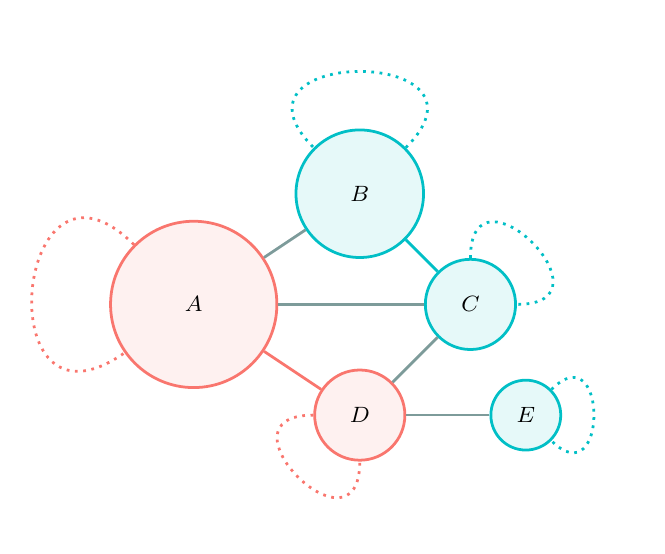
\begin{tikzpicture}[x=2em,y=2em,line width=1pt]
  \footnotesize
  \useasboundingbox (-6,-4) rectangle (+5,+5);
  \node[FSA={5*sqrt(17em)}{G1}](a) at (-3, 0) {$A$};
  \node[FSA={5*sqrt(10em)}{G2}](b) at ( 0,+2) {$B$};
  \node[FSA={5*sqrt( 5em)}{G2}](c) at (+2, 0) {$C$};
  \node[FSA={5*sqrt( 5em)}{G1}](d) at ( 0,-2) {$D$};
  \node[FSA={5*sqrt( 3em)}{G2}](e) at (+3,-2) {$E$};
  \draw[G1,dotted](a) edge[out=135,in=215,looseness=4] (a);
  \draw[G2,dotted](b) edge[out= 45,in=135,looseness=4] (b);
  \draw[G2,dotted](c) edge[out= 90,in=360,looseness=4] (c);
  \draw[G1,dotted](d) edge[out=180,in=270,looseness=4] (d);
  \draw[G2,dotted](e) edge[out= 45,in=315,looseness=4] (e);
  \draw[G3](a) edge (b);
  \draw[G3](a) edge (c);
  \draw[G1](a) edge (d);
  \draw[G2](b) edge (c);
  \draw[G3](c) edge (d);
  \draw[G3](d) edge (e);
\end{tikzpicture}